\subsection{Open Event Machine}
Open Event Machine is a runtime system for multicore platforms originally developed by NSN for the network dataplane. OpenEM is used to write dynamically load balanced applications with run-to-completion principle.

The key concepts of OpenEM are events, execution objects, queues and the scheduler. \textbf{Event} is the unit of communication in OpenEM. Events are typically used to carry data to be processed but can be data-less tokens as well. The event descriptors are allocated at the initialization of the Queues. \textbf{Execution objects} encapsulate the algorithm to execute when an event is received. \textbf{Queues} connect events (data) and execution objects (algorithms). Each queue is associated with one execution object and all queued events will be processed by this execution object. \textbf{Scheduler} moves allocated events to queues. \textbf{Dispatcher} is called by the user in a dispatch loop. Dispatcher calls the ‘receive’ function of the execution object of the connected queue.

\subsection{Texas Instruments Implementation of OpenEM}
The Texas Instruments implementation of Open Event Machine runtime system is included in the MCSDK (chapter \ref{MCSDK}). OpenEM version 1.0.0.2 is used in the experiment.

The OpenEM library is OS agnostic: the OpenEM dispatcher can be called from bare metal software or from an OS thread. The TI implementation of OpenEM Leverages the Multicore Navigator for hardware queues and packet communication. The scheduler always runs on a PDSP core and is defined by firmware specific to OpenEM.

The OpenEM execution model is described in figure \ref{tiem}. The event descriptors are allocated at OpenEM initialization in the free pool. The application allocates events from the free pool using \textit{em\_alloc}. Events can be allocated either at runtime or at initialization. After the allocated event has been populated it is sent to a queue using \textit{em\_send}. The queues are associated with specific execution objects at initialization and therefore they determine which EO will process the events the queues. The scheduler running on a PDSP core (chapter \ref{navigator}) manages the queues (virtual queues mapped to QMSS hardware queues). The scheduling operations are carried out on an explicit request from a DSP core when a call to \textit{ti\_em\_preschedule} is made. When one of the cores mapped to a specific execution object finishes executing its current event it makes a call to \textit{ti\_em\_dispatch\_once} which triggers a call to the \textit{receive} function of the execution object. The execution object processes the data and makes a call to \textit{em\_free} to return the event to its free pool.
\begin{figure}[h!]
\begin{center}
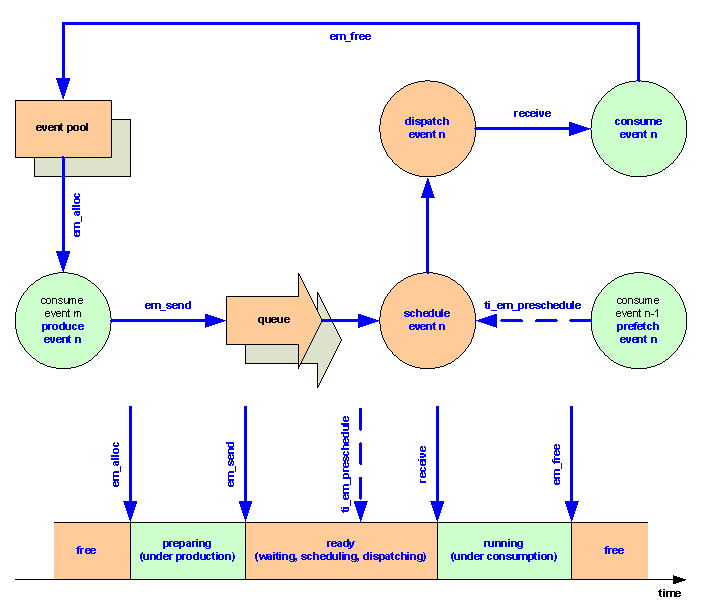
\includegraphics[width=1.3\textwidth,natwidth=701,natheight=500]{openem_model.png}
\caption{The OpenEM execution model}\label{tiem}
\end{center}
\end{figure}

The concept of queue groups is used to specify which cores can execute which EOs. Queues are associated with EOs and each queue belongs to a queue group. Queue groups define which cores can execute the events from the queues in the group using a core mask.

The scheduler running on a PDSP core considers four scheduling criteria: \textbf{Priority}, \textbf{Atomicity}, \textbf{Locality} and \textbf{Order}. Each queue has a priority. The scheduler will always select events from queues with the highest priority. Queues are either atomic or parallel. Events from parallel queues can be scheduled on as many cores as are available for the queue. In contrast no event from an atomic queue can be scheduled while another event from the same queue is executing. The scheduler tries to schedule events from certain queues on the same cores if possible. The last criterion for scheduling is order. If multiple events are eligible for scheduling, the event that has been in a queue longest will be scheduled.

\textbf{Texas Instrument} OpenEM White Paper, ti.openem.white.paper.pdf\\
\textbf{Texas Instrument} OpenEM User Guide, ti.openem.user.guide.pdf\\
\textbf{Texas Instrument} OpenEM Api Guide, ti.openem.api.guide.pdf\\